\section{Konzept}

Diese Sektion enthält eine Beschreibung des generellen Lösungsansatzes, der in
den einzelnen Phasen des Programmes verfolgt wird. Eine detaillierte Dokumentation
der konkreten Umsetzung befindet sich in Sektion \ref{module} - Modulbeschreibung.

Um eine hohe Erkennungsrate der Captchas zu erreichen und den Rechenaufwand
gering zu halten, haben wir uns dazu entschieden
uns nicht ausschließlich auf die Funktion des neuronalen Netzes zu verlassen
und stattdessen im Programmablauf Vorbereitungsphasen zu integrieren, die die
Daten für das neuronale Netz aufbereiten. Durch diese Aufbereitung wollen wir
die Zahl der Inputneuronen gering halten und eventuelle Störsignale bereits Image
Voraus entfernen.

Aufgrund dieser Anforderungen haben wir uns bei der Umsetzung für Matlab entschieden, 
da es bereits passende Erweiterungen zur Aufbereitung von Bildern und zum
Erstellen von neuronalen Netzen speziell für die Mustererkennung bietet.


\subsection{Ablaufphasen des Programms}

Der Ablauf des Programms kann in folgende grobe Phasen unterteilt werden: 

\begin{itemize}

\item Trainingsphase

Erstellen des neuronalen Netzes.


\item Einlesen und Aufbereiten der Captchas

Liest die Captchas aus den Dateien ein und entfernt grobe Störsignale.


\item Segmentierung

Teilt die aufbereiteten Bilder in einzelne Zeichen und normalisiert die
Ausrichtung.


\item Datenaggregation

Zusammenfassen von verwandten Datensätzen um die Anzahl der Eingaben zu reduzieren.


\item Klassifizierung

Erkennen der Zeichen durch das neuronale Netz

\end{itemize}


\subsubsection{Trainingsphase}

Die Trainingsphase ist die Phase in der ein neuronales Netz zum Erkennen der
Zeichen erstellt wird. Die Trainingsphase soll nur dann aufgerufen werden, wenn
nicht bereits ein Vorbereitetes Netz existiert. In der Trainingsphase werden
vorbereitete Captchas zusammen mit der Lösung eingelesen und analog zu den
normalen Bildern aufbereitet. Die einzelnen Zeichen werden zusammen mit dem
Ergebnis zum Trainieren des Neuronalen Netzes verwendet. Die Trainingsphase
soll so lange andauern, bis sich zwischen den einzelnen Trainingsphasen keine
relevante Verbesserung ergibt.

\subsubsection{Einlesen und Aufbereiten der Captchas}

\begin{wrapfigure}[6]{r}{5cm}
  \begin{center}
  \vspace{-48pt}
    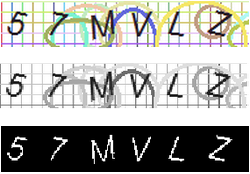
\includegraphics[width=4cm]{res/Aufbereitung.png}
  \end{center}
  \caption{Aufbereitung eines Captchas}
\end{wrapfigure}

In diesem Schritt werden alle Bilder aus einem Eingabeverzeichnis eingelesen und
aufbereitet. Die Aufbereitung versucht alle Pixel, die nicht zum eigentlichen
Text gehören herauszufiltern. Zudem werden Farben durch binäre Werte ersetzt
die entweder Schwarz oder Weiß darstellen. Hierbei wird anhand eines
Schwellwertes unterschieden ab wann ein Graustufenwert als Schwarz oder als
Weiß gilt. Eine genauere Beschreibung der Aufarbeitung der Bilder befindet sich
in Kapitel \ref{images} - Aufbereitung von Bildern mit der Matlab-Image-Toolbox.


\subsubsection{Segmentierung}

  \begin{wrapfigure}[6]{R}[0pt]{6cm}
  \vspace{-35pt}
  \begin{center}
    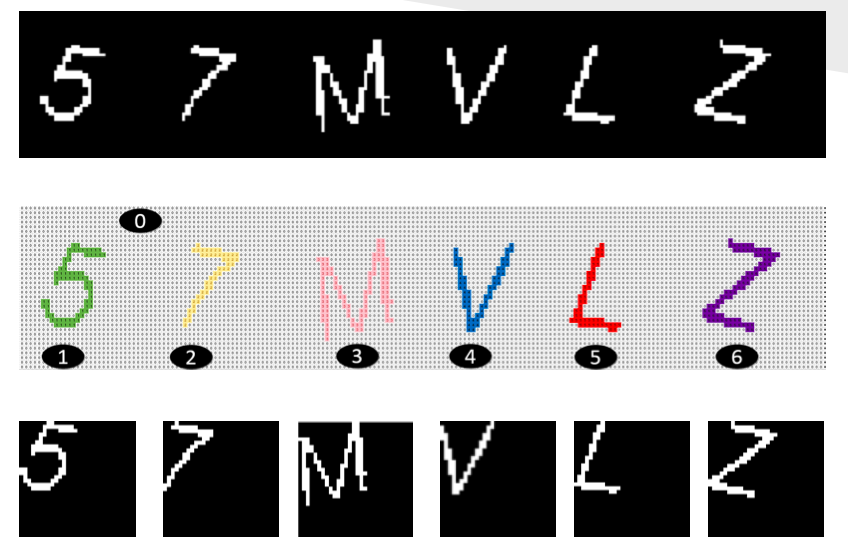
\includegraphics[width=5cm]{res/Segmentierung.png}
  \end{center}
  \vspace{-5pt}
  \caption{Segmentierung}
  \vspace{-10pt}
\end{wrapfigure}


Bei der Segmentierung wird versucht die Zeichen des Worts in einzelne Segmente
zu unterteilen. Da das neuronale Netz eine konstante Menge an Eingabewerten
benötigt, wird zudem die Auflösung der Segmente auf eine Einheitliche größe
Festgelegt. Alle Zeichen werden auf die gleiche Art ausgerichtet um
Verschiebungen auszugleichen.

\subsubsection{Datenaggregation}

\begin{wrapfigure}[15]{R}[0pt]{7cm}
  \begin{center}
    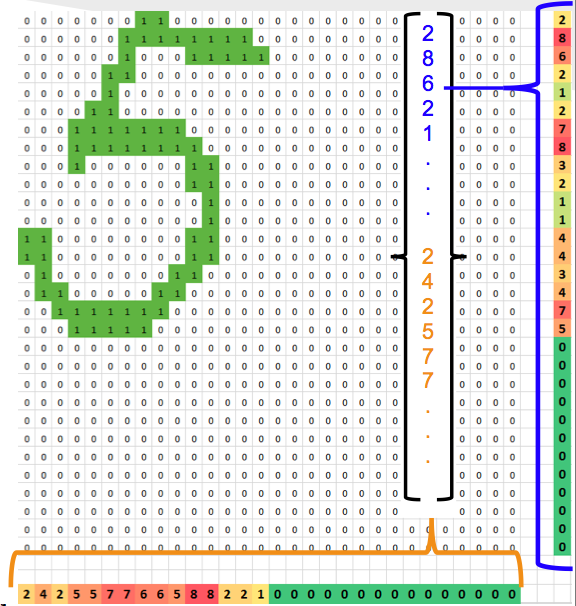
\includegraphics[width=6cm]{res/Aggregation.png}
  \end{center}
  \vspace{-5pt}
  \caption{Aggregation der Spalten/Zeilen}
  \vspace{-10pt}
\end{wrapfigure}


Bei der Datenaggregation wird versucht die Menge an Eingabewerten zu reduzieren,
ohne dabei viel Genauigkeit zu verlieren. Dies wird erreicht indem 
die Summen aller Schwarzen Pixel pro Zeile und Spalte gebildet wird. 

Ohne diese Aggregation, also bei direkter Eingabe aller Pixel in das
neuronale Netz, wäre die Laufzeit des Lernvorgangs und der Mustererkennung zu
hoch um das Programm sinnvoll verwenden zu können.
\subsubsection{Klassifizierung}

Die Klassifizierung benutzt das neuronale Netz, um die eigentliche
Mustererkennung durchzuführen und so die einzelnen Buchstaben zu
erkennen. Jede Summe aus der Datenaggregation wird als einzelner Eingabewert
für das Netz verwendet. Diese Werte sollen in Matlab in Form eines Vektors zu
einem Set aus Eingabewerten für ein einzelnes Zeichen zusammengefasst werden.

\section{Struktur des neuronalen Netzes}

\begin{wrapfigure}[15]{R}[0pt]{7cm}
  \begin{center}
    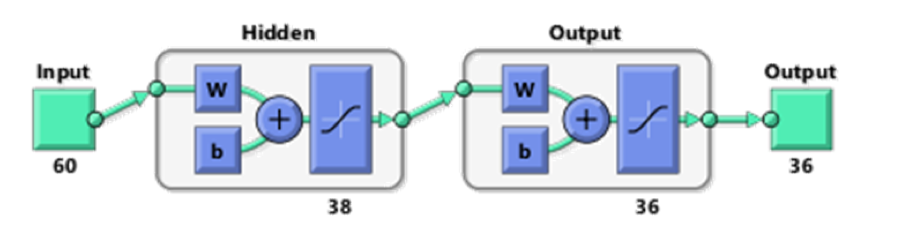
\includegraphics[width=12cm]{res/PatternNet-Aufbau.png}
  \end{center}
  \vspace{-5pt}
  \caption{Aufbau des Neuronalen Netzes}
  \vspace{-10pt}


\end{wrapfigure}
Um festzustellen wie viele Hidden-Neuronen das Netz braucht, wurde die Leistungsfähigkeit des Netzes bei verschiedensten Mengen an Neuronen getestet. Da der Anstieg der Leistungsfähigkeit ab $38$ Hidden-Neuronen aufhört, legen wir die Anzahl dieser auf $38$ fest.

\subsection{Matlab - Die Klasse ``Patternnet''}

In der Matlab-Toolbox für neuronale Netze existiert bereits ein vorgefertigtes
neuronales Netz für die Mustererkennung. Diese Klasse nennt sich ``Patternnet''
und erbt von der Basisklasse ``nnet''. Die Klasse erstellt ein Feedforward-Netz
mit der Lernfunktion ``trainscg'', die die Skalierte Gradientenmethode zum
Berechnen der Extrema verwendet.


\subsection{Transferfunktion}
 Als Transferfunktion wird die Funktion``tansig'' verwendet, die eine Gleichung der folgenden Form darstellt:

\begin{equation}
n = tansig(n) =  \frac{2}{(1 + e^{-2*n})} - 1
\end{equation}

\subsection{Skalierte Gradientenmethode}

Die Skalierte Gradientenmethode wird verwendet um die Gewichtungen der
Transferfunktion zu aktualisieren. 

\newpage
\section{Aufbereitung von Bildern mit der Matlab-Image-Toolbox}
\label{images}
